\chapter{Discussion}
\label{cha:discussion}
klustering av rörelsemönster
mängden data som används, inducing inputs


% This chapter contains the following sub-headings.

% \section{Results}
% \label{sec:discussion-results}

% Are there anything in the results that stand out and need be
% analyzed and commented on? How do the results relate to the
% material covered in the theory chapter? What does the theory
% imply about the meaning of the results? For example, what
% does it mean that a certain system got a certain numeric value
% in a usability evaluation; how good or bad is it? Is there
% something in the results that is unexpected based on the
% literature review, or is everything as one would theoretically
% expect?

\section{Method}\label{sec:discussion-method}
This section addresses the method used and its flaws.

\subsection{Maximum Likelihood Estimation}
ML-estimated models are typically prone to overfitting, and attempts were made to
MAP-estimate them. The kernel parameters were modeled as 
$\ell \sim \Gamma(\alpha_\ell, \beta_\ell)$, $\var \sim \Gamma(\alpha_\var, \beta_\var)$, 
$\var_b \sim \Gamma(\alpha_{\var_b}, \beta_{\var_b})$, and were
estimated by fitting distributions to populations of ML-estimated parameters of 100 trajectories set
aside solely for this purpose; the models were never presented with these
trajectories during training or testing. An illustration of 
the parameters estimation can be seen in Figure~\ref{fig:seg-state-model-priors}.
\begin{figure}
  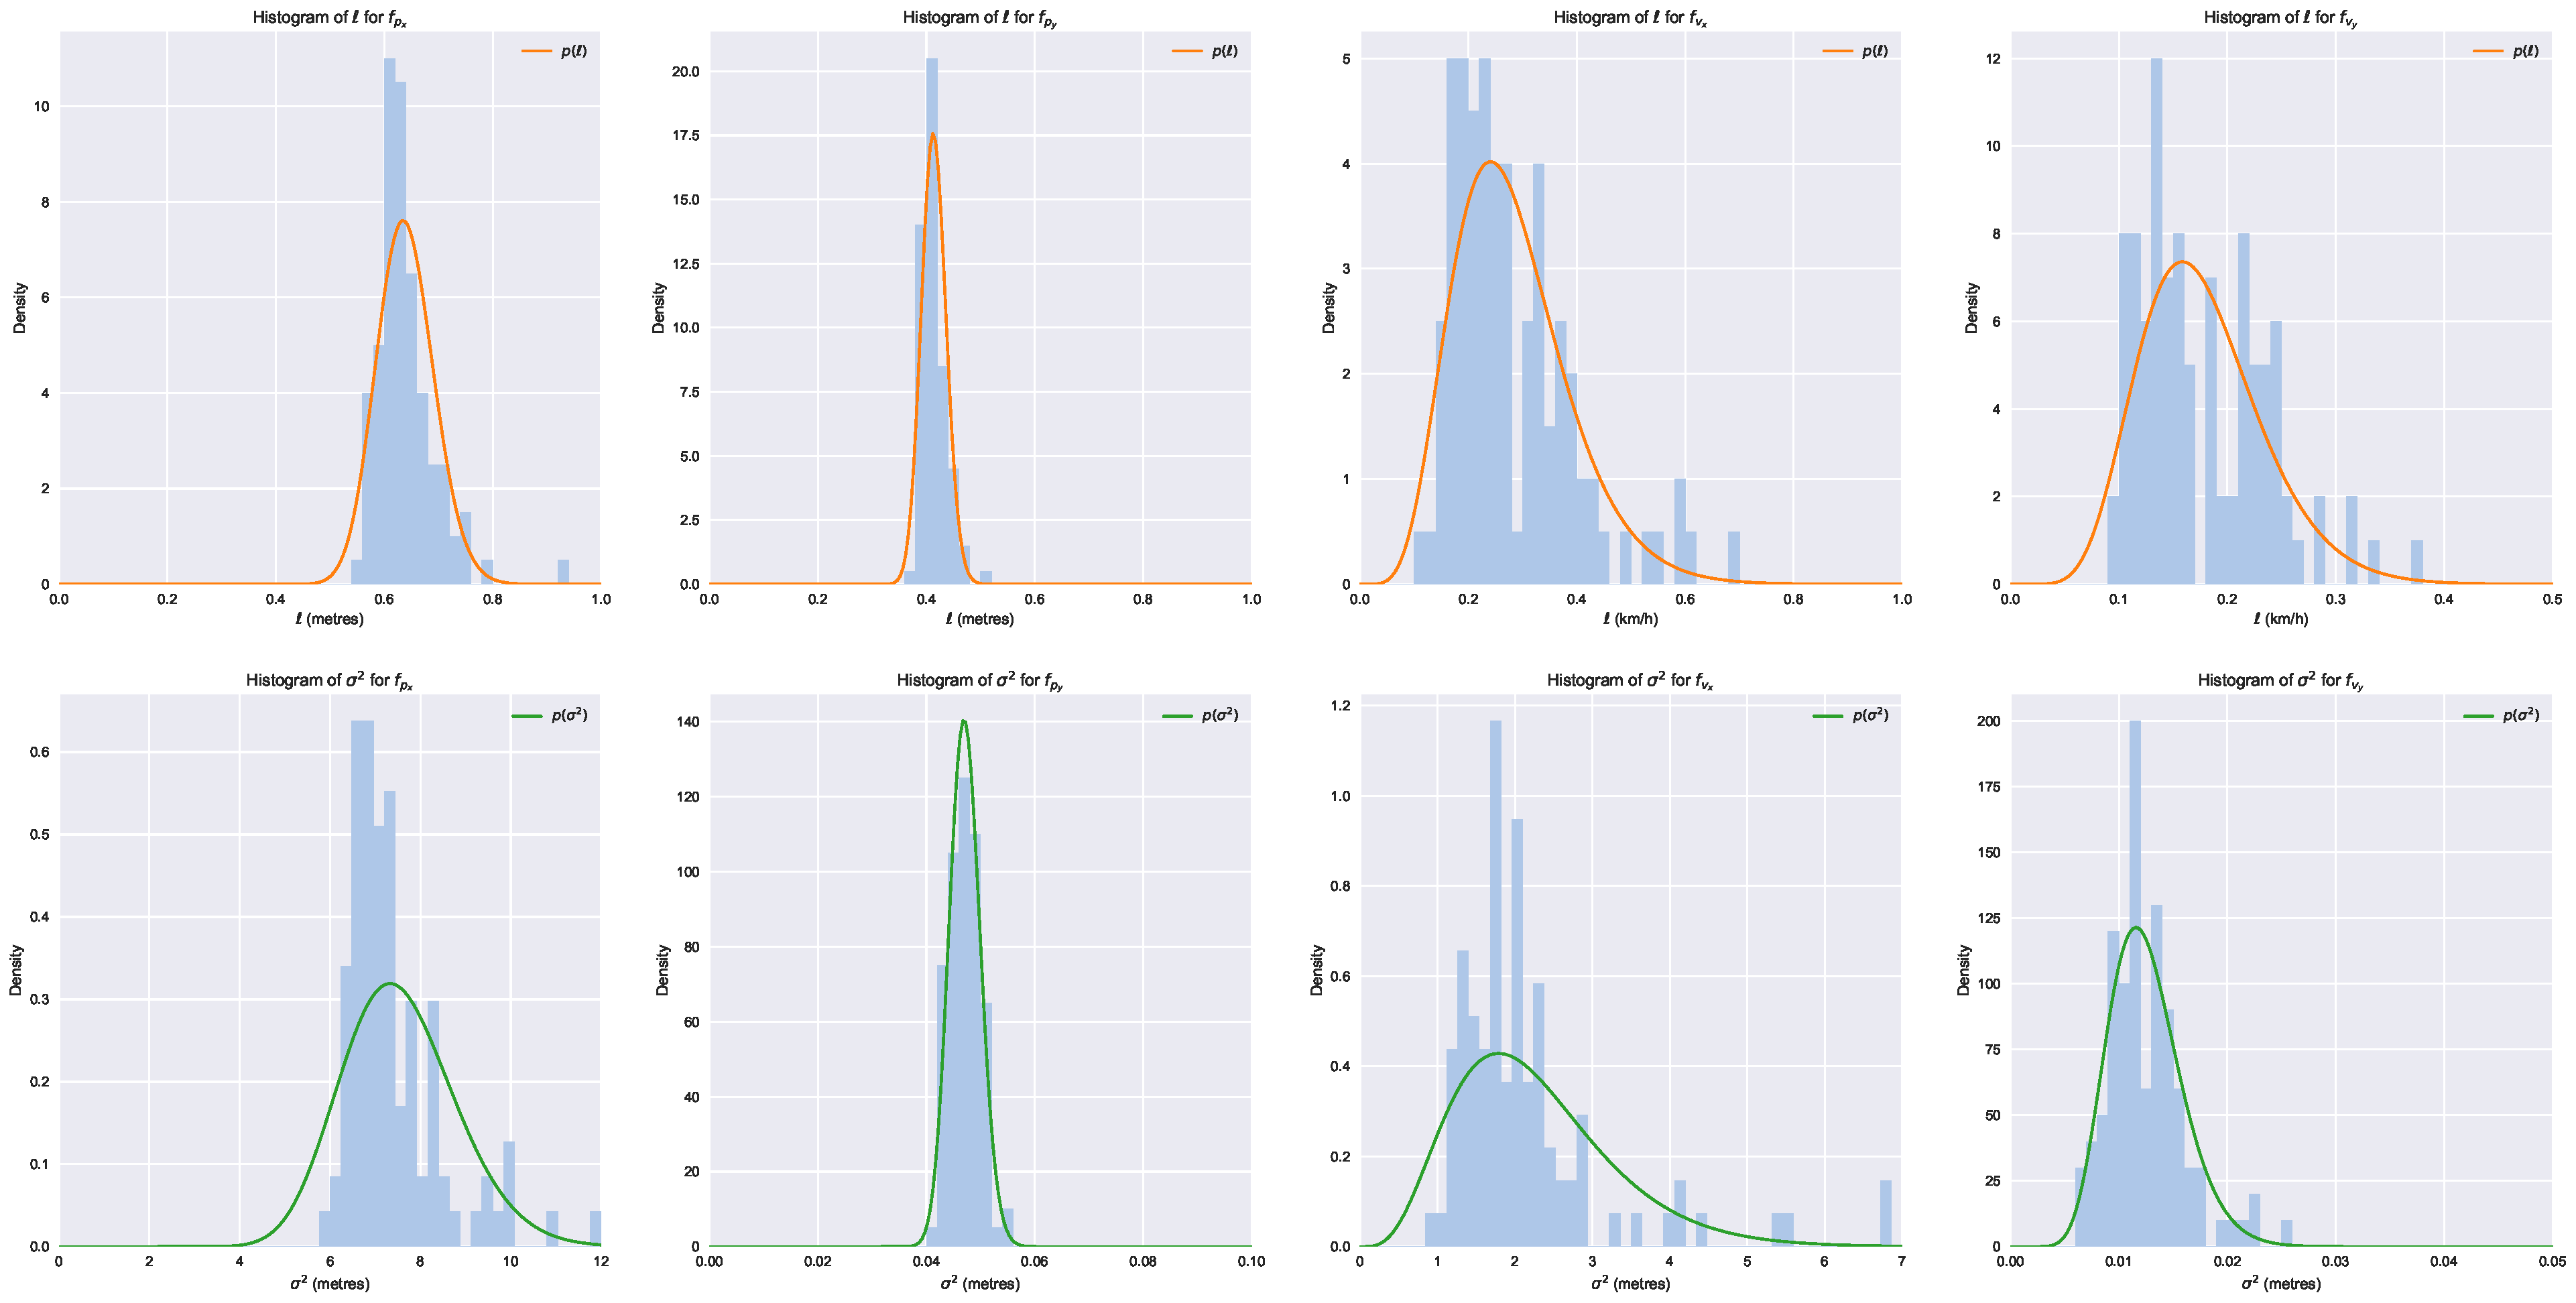
\includegraphics[scale=0.48,width=\textwidth]{seg-1-state-model-priors}
  \caption{Plots of estimated prior parameters from state models for
    segmeent one (Parameters of $\synchf$ and $\predf$ are not
    shown). The histograms show the parameter distributions from
    the learned trajectory models, and the Gamma distributions show
    the estimated priors.}\label{fig:seg-state-model-priors}
\end{figure}
Using MAP-estimation did however have a much greater regularising
effect than desired. Since the project considered single-trajectory
motion patterns the characteristics of a single trajectory was
paramount to be able to identify it. Paradoxically, this means that
over-fitting was \textit{good} for the model; regularisation caused
the differences in models to be ``smoothed out'', making it hard for
the model to tell them apart.

\subsection{Low Sample Sizes}
The project did use a fairly low amount of trajectories for its
evaluation. The simple reason for this is time constraints; evaluating
the model performance on only 50 trained models took over two hours.
Attempts were made to use SGPs for all functions, which would have made
computing model posteriors much faster and enabled training and
evaluating on a larger data set, but this had a
large regularising effect akin to MAP-estimation, as illustrated in Figure~\ref{fig:inducing-inputs-regularisation}.

\subsection{Unrepresentative Samples}
Using only data from a single bus line is of course hardly
representative of the greater population of bus lines. <inte
klar. kanske mät lite olika saker för olika buslinjer för att jämföra>

\begin{figure}
  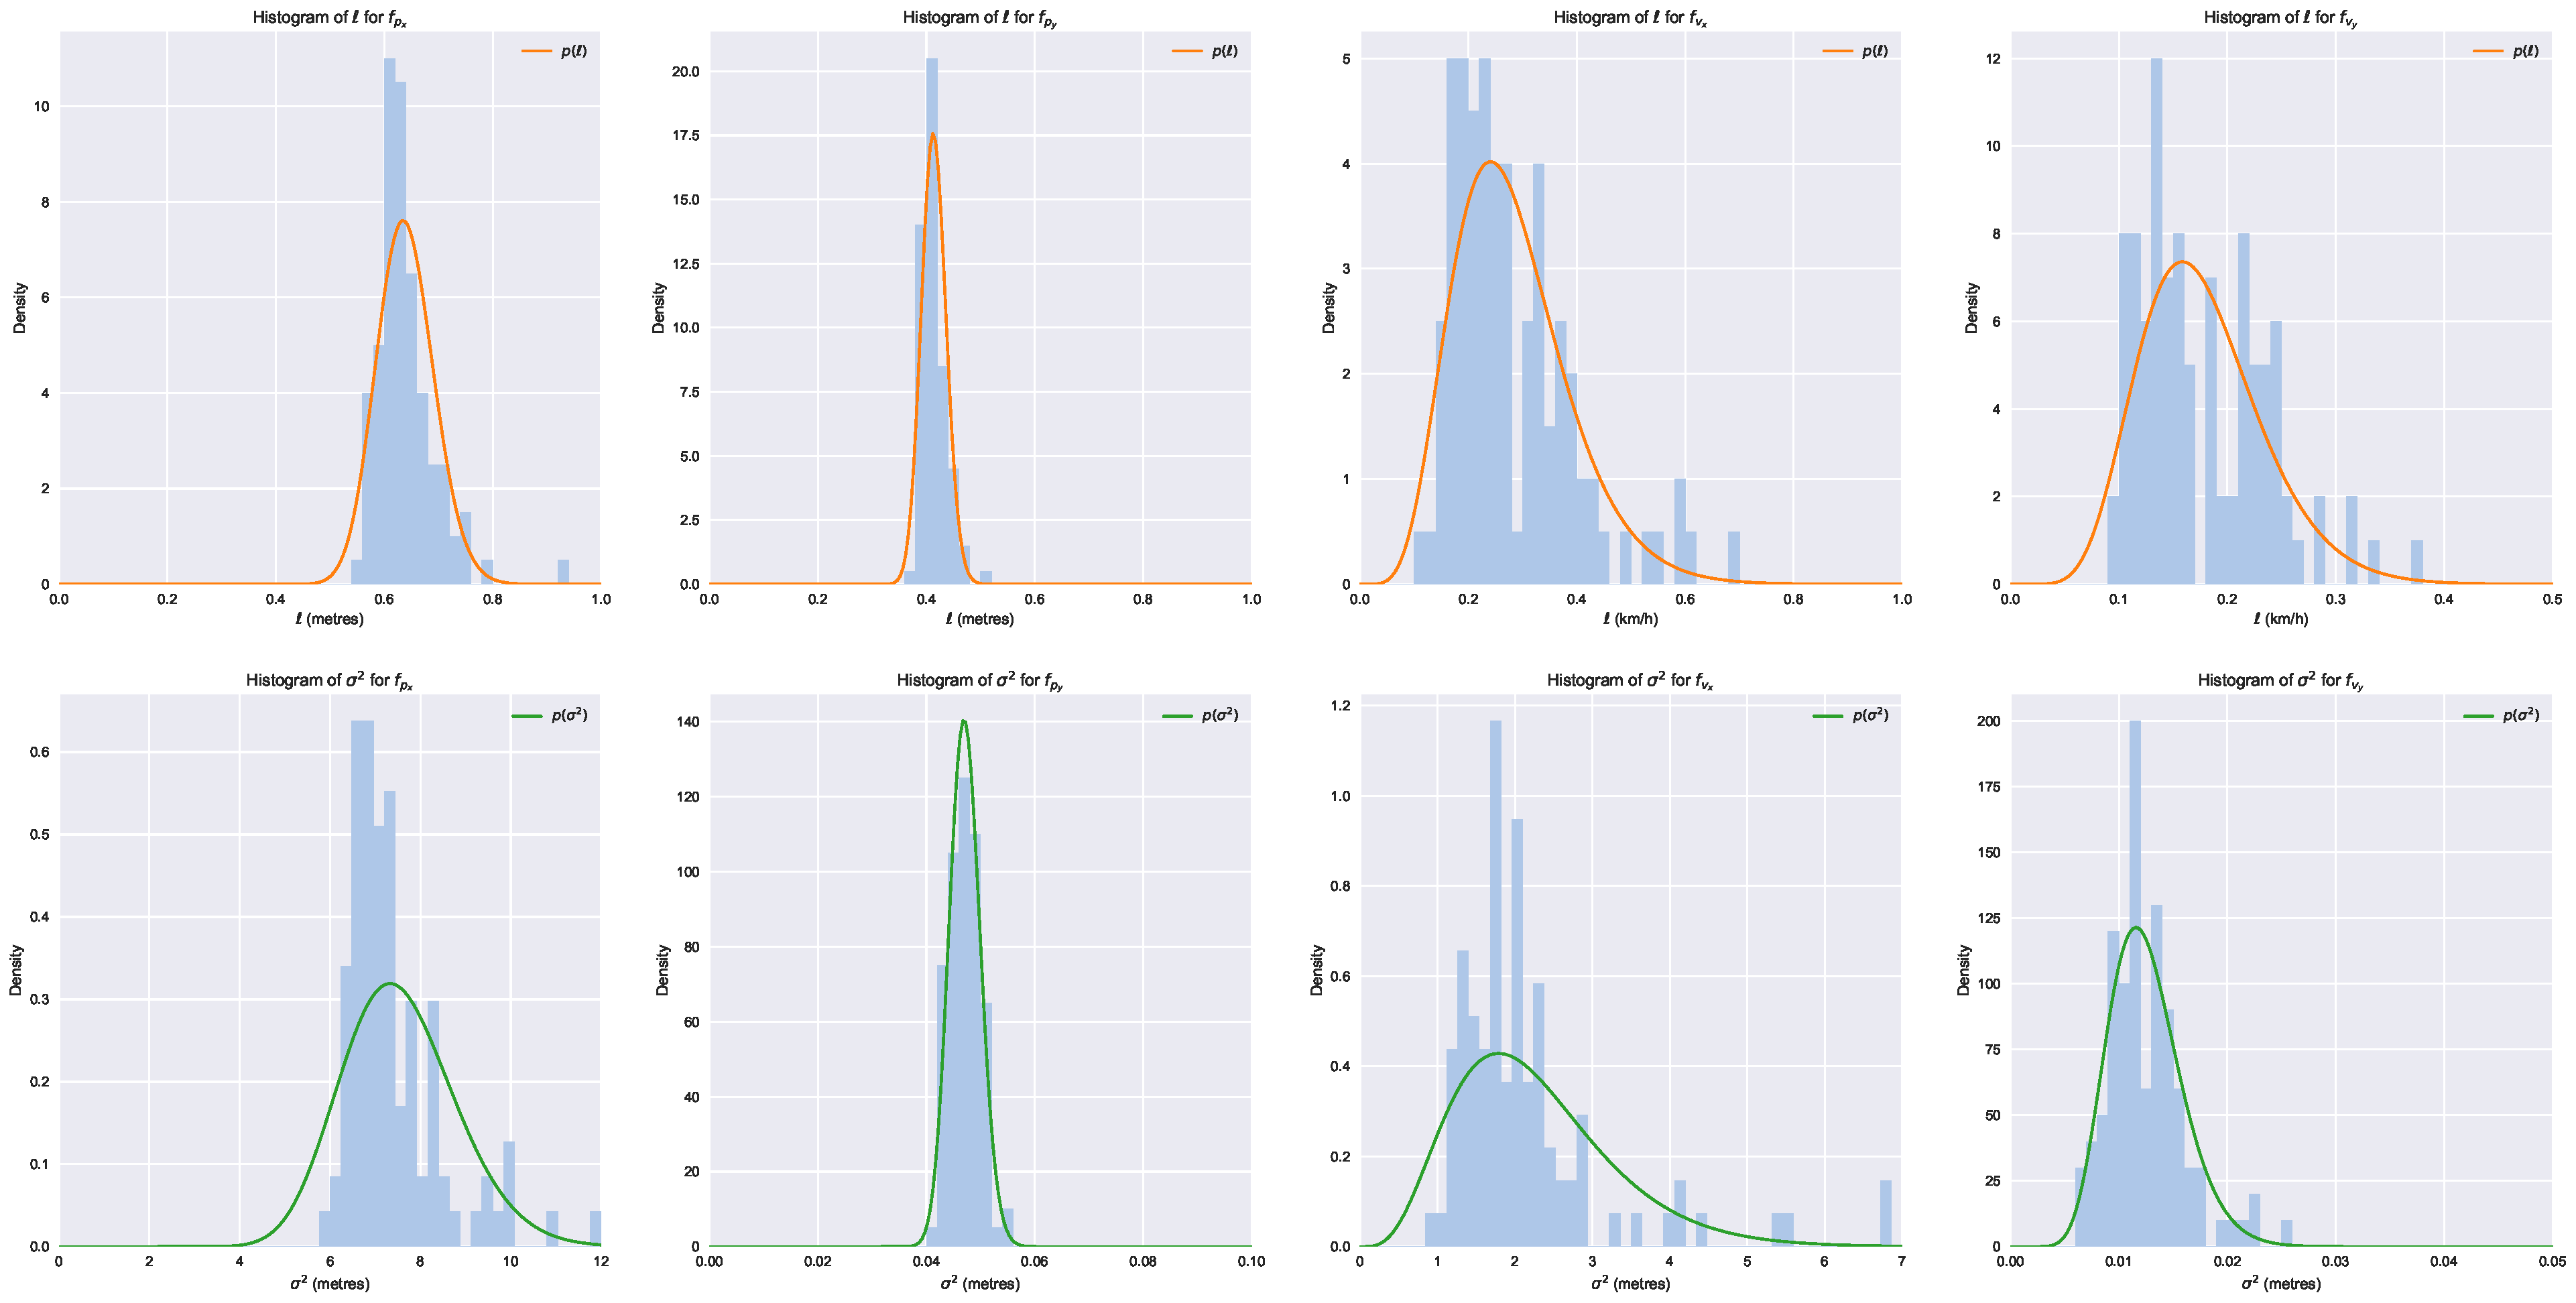
\includegraphics[scale=0.48,width=\textwidth]{seg-1-state-model-priors}
  \caption{PLACEHOLDER - will describe regularisation induced by
    inducing inputs.}\label{fig:inducing-inputs-regularisation}
\end{figure}

% This is where the applied method is discussed and criticized.
% Taking a self-critical stance to the method used is an
% important part of the scientific approach.

% A study is rarely perfect. There are almost always things one
% could have done differently if the study could be repeated or
% with extra resources. Go through the most important
% limitations with your method and discuss potential
% consequences for the results. Connect back to the method
% theory presented in the theory chapter. Refer explicitly to
% relevant sources.

% The discussion shall also demonstrate an awareness of methodological
% concepts such as replicability, reliability, and validity. The concept
% of replicability has already been discussed in the Method chapter
% (\ref{cha:method}). Reliability is a term for whether one can expect
% to get the same results if a study is repeated with the same method. A
% study with a high degree of reliability has a large probability of
% leading to similar results if repeated. The concept of validity is,
% somewhat simplified, concerned with whether a performed measurement
% actually measures what one thinks is being measured. A study with a
% high degree of validity thus has a high level of credibility. A
% discussion of these concepts must be transferred to the actual context
% of the study.

% The method discussion shall also contain a paragraph of
% source criticism. This is where the authors’ point of view on
% the use and selection of sources is described.

% In certain contexts it may be the case that the most relevant
% information for the study is not to be found in scientific
% literature but rather with individual software developers and
% open source projects. It must then be clearly stated that
% efforts have been made to gain access to this information,
% e.g. by direct communication with developers and/or through
% discussion forums, etc. Efforts must also be made to indicate
% the lack of relevant research literature. The precise manner
% of such investigations must be clearly specified in a method
% section. The paragraph on source criticism must critically
% discuss these approaches.

% Usually however, there are always relevant related research.
% If not about the actual research questions, there is certainly
% important information about the domain under study.

% \section{The work in a wider context}
% \label{sec:work-wider-context}

% There must be a section discussing ethical and societal
% aspects related to the work. This is important for the authors
% to demonstrate a professional maturity and also for achieving
% the education goals. If the work, for some reason, completely
% lacks a connection to ethical or societal aspects this must be
% explicitly stated and justified in the section Delimitations in
% the introduction chapter.

% In the discussion chapter, one must explicitly refer to sources
% relevant to the discussion.
